\documentclass[landscape,final]{baposter}

\usepackage[-1]{pagesel} % limit to one page

\usepackage{times}
\usepackage{calc}
\usepackage{graphicx}
\usepackage{amsmath}
\usepackage{amssymb}
\usepackage{relsize}
\usepackage{multirow}
\usepackage{bm}
\usepackage{epstopdf}
\usepackage{setspace}
\usepackage{graphicx}
\graphicspath{{images/}}
\usepackage{multicol}
\usepackage{mathtools,bm}
\usepackage{vwcol}

\usepackage{pgfbaselayers}
\pgfdeclarelayer{background}
\pgfdeclarelayer{foreground}
\pgfsetlayers{background,main,foreground}

\usepackage{helvet}
%\usepackage{bookman}
\usepackage{palatino}



\newcommand{\captionfont}{\footnotesize}

\selectcolormodel{cmyk}

%\graphicspath{{images/}}

%\graphicspath{{figures/}}



%%%%%%%%%%%%%%%%%%%%%%%%%%%%%%%%%%%%%%%%%%%%%%%%%%%%%%%%%%%%%%%%%%%%%%%%%%%%%%%%
%%%% Some math symbols used in the text
%%%%%%%%%%%%%%%%%%%%%%%%%%%%%%%%%%%%%%%%%%%%%%%%%%%%%%%%%%%%%%%%%%%%%%%%%%%%%%%%

\newcommand{\CC}{\mathbb{C}}
\newcommand{\RR}{\mathbb{R}}
\newcommand{\LL}{\mathcal{L}}
\newcommand{\OO}{\mathcal{O}}

\newcommand{\veca}{\vec{a}}
\newcommand{\vecb}{\vec{b}}
\newcommand{\vecd}{\vec{d}}
\newcommand{\vece}{\vec{e}}
\newcommand{\vecf}{\vec{f}}
\newcommand{\vecn}{\vec{n}}
\newcommand{\vecp}{\vec{p}}
\newcommand{\vecr}{\vec{r}}
\newcommand{\vecu}{\vec{u}}
\newcommand{\vecv}{\vec{v}}
\newcommand{\vecw}{\vec{w}}
\newcommand{\vecx}{\vec{x}}
\newcommand{\vecy}{\vec{y}}
\newcommand{\vecz}{\vec{z}}


\renewcommand{\vec}[1]{\mathbf{#1}}

%%%%%%%%%%%%%%%%%%%%%%%%%%%%%%%%%%%%%%%%%%%%%%%%%%%%%%%%%%%%%%%%%%%%%%%%%%%%%%%%
% Multicol Settings
%%%%%%%%%%%%%%%%%%%%%%%%%%%%%%%%%%%%%%%%%%%%%%%%%%%%%%%%%%%%%%%%%%%%%%%%%%%%%%%%
\setlength{\columnsep}{0.7em}
\setlength{\columnseprule}{0mm}


%%%%%%%%%%%%%%%%%%%%%%%%%%%%%%%%%%%%%%%%%%%%%%%%%%%%%%%%%%%%%%%%%%%%%%%%%%%%%%%%
% Save space in lists. Use this after the opening of the list
%%%%%%%%%%%%%%%%%%%%%%%%%%%%%%%%%%%%%%%%%%%%%%%%%%%%%%%%%%%%%%%%%%%%%%%%%%%%%%%%
\newcommand{\compresslist}{%
\setlength{\itemsep}{1pt}%
\setlength{\parskip}{0pt}%
\setlength{\parsep}{0pt}%
}

\usepackage{enumitem}
\setlist[itemize,1]{leftmargin=\dimexpr 26pt-0.22in}

\DeclareMathSizes{10}{9}{7}{6}
\DeclareSymbolFont{extraup}{U}{zavm}{m}{n}
\DeclareMathSymbol{\vardiamond}{\mathalpha}{extraup}{87}

\newcommand{\headshotsize}{1.25in}




%%%%%%%%%%%%%%%%%%%%%%%%%%%%%%%%%%%%%%%%%%%%%%%%%%%%%%%%%%%%%%%%%%%%%%%%%%%%%%
%%% Begin of Document
%%%%%%%%%%%%%%%%%%%%%%%%%%%%%%%%%%%%%%%%%%%%%%%%%%%%%%%%%%%%%%%%%%%%%%%%%%%%%%

\begin{document}

%%%%%%%%%%%%%%%%%%%%%%%%%%%%%%%%%%%%%%%%%%%%%%%%%%%%%%%%%%%%%%%%%%%%%%%%%%%%%%
%%% Here starts the poster
%%%---------------------------------------------------------------------------
%%% Format it to your taste with the options
%%%%%%%%%%%%%%%%%%%%%%%%%%%%%%%%%%%%%%%%%%%%%%%%%%%%%%%%%%%%%%%%%%%%%%%%%%%%%%
\typeout{Poster Starts}
%\background{
%  \begin{tikzpicture}[remember picture,overlay]%
%    \draw (current page.north west)+(-2em,-0em) node[anchor=north west] {\hspace{-2em}\includegraphics[height=1.1\textheight]{silhouettes_background}};
%  \end{tikzpicture}%
%}

\definecolor{cuGold}{cmyk}{0, .10, .48, .22}
\definecolor{cuBlack}{cmyk}{0, 0, 0, 1.00}
\definecolor{cuDarkGray}{cmyk}{.38, .28, .21, .63}
\definecolor{cuLightGray}{cmyk}{.16, .11, .11, .29}

\begin{poster}{
	% Show grid to help with alignment
	grid=no,
	columns=4,
	% Column spacing
	colspacing=1em,
	% Color style
	bgColorOne=cuBlack,
	bgColorTwo=cuBlack,
	borderColor=cuGold,
	headerColorOne=cuDarkGray,
	headerColorTwo=black,
	headerFontColor=white,
	%  headerFontColor=black,
	%  boxColorOne=lightestblue,
	%  boxColorTwo=lightestblue,
	boxColorOne=white,
	boxColorTwo=white,
	% Format of textbox
	%textborder=roundedleft,
	textborder=rounded,
	% Format of text header
	eyecatcher=yes,
	headerborder=closed,
	headerheight=0.11\textheight,
	%  headershape=rectangle,
	headershape=rounded,
	headershade=plain,
	headerfont=\Large\textsf, %Sans Serif
	boxshade=plain,
	%  background=shade-tb,
	background=plain,
	linewidth=2pt
}
% Eye Catcher
{{\begin{minipage}{5in}

\includegraphics[height=10em]{cu_logo}
%%%%%%%%%%%%%%%%%%%%%%%%%%%%%%%%%%%%%%%%%%%%%%%%%%%%%%%%%%%%%%%%%%%%%%%%%%%%%%%%%%%%%%%%%%
\end{minipage}}} % No eye catcher for this poster. If an eye catcher is present, the title is centered between eye-catcher and logo.
% Title
{
	\bf \huge
	\color{cuGold}
	Input-Response Relations for Traveling Waves\\in Neural Fields with Synaptic Depression
	\vspace{1mm}
}
% Authors
{\sc\large 
\color{cuGold}
	Sage B. Shaw and Zachary P. Kilpatrick\\ University of Colorado Boulder
}
% University logo 
{{\begin{minipage}{5in}
\vfill  
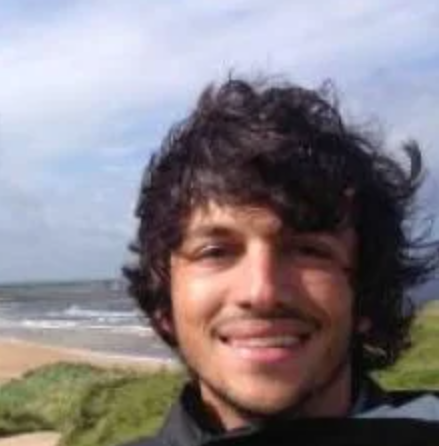
\includegraphics[height=\headshotsize]{headshot_zack}
\hspace{.5cm}

\includegraphics[height=\headshotsize]{headshot_sage}
\hspace{.5cm}

\includegraphics[height=\headshotsize]{QR}
\end{minipage}}}

%\tikzstyle{light shaded}=[top color=baposterBGtwo!30!white,bottom color=baposterBGone!30!white,shading=axis,shading angle=30]

  % Width of left inset image
     \newlength{\leftimgwidth}
     \setlength{\leftimgwidth}{0.78em+8.0em}

%%%%%%%%%%%%%%%%%%%%%%%%%%%%%%%%%%%%%%%%%%%%%%%%%%%%%%%%%%%%%%%%%%%%%%%%%%%%%%
%%% Now define the boxes that make up the poster
%%%---------------------------------------------------------------------------
%%% Each box has a name and can be placed absolutely or relatively.
%%% The only inconvenience is that you can only specify a relative position 
%%% towards an already declared box. So if you have a box attached to the 
%%% bottom, one to the top and a third one which should be in between, you 
%%% have to specify the top and bottom boxes before you specify the middle 
%%% box.
%%%%%%%%%%%%%%%%%%%%%%%%%%%%%%%%%%%%%%%%%%%%%%%%%%%%%%%%%%%%%%%%%%%%%%%%%%%%%%
    %
    % A coloured circle useful as a bullet with an adjustably strong filling
    \newcommand{\colouredcircle}[1]{%
      \tikz{\useasboundingbox (-0.2em,-0.32em) rectangle(0.2em,0.32em); \draw[draw=black,fill=baposterBGone!80!black!#1!white,line width=0.03em] (0,0) circle(0.18em);}}

%%%%%%%%%%%%%%%%%%%%%%%%%%%%%%%%%%%%%%%%%%%%%%%%%%%%%%%%%%%%%%%%%%%%%%%%%%%%%%
\headerbox{Summary}{name=summary,column=0,row=0}{
	 \textbf{Scientific Question:} How do brains encode and predict motion? \\
	 \textbf{Bottom Up Approach:} One dimensional neural-field models can admit traveling fronts/pulses. How do these solutions react to external stimulation, and can they be used to encode the velocity of moving objects?
	 \vspace{.2cm}
}

%%%%%%%%%%%%%%%%%%%%%%%%%%%%%%%%%%%%%%%%%%%%%%%%%%%%%%%%%%%%%%%%%%%%%%%%%%%%%%
\headerbox{Neural-Field Model}{name=model,column=0, below=summary, above=bottom}
{
	Neural tissues are composed of cells called neurons, which are connected to eachother through synapses forming a network. These networks can be quite large we approximate them with a system of integro-differential equations called a \textit{neural-field model}. Our model incorporates \textit{synaptic plasticity} - a phenomenon where the strength of synaptic connections changes due to availability of synaptic resources. We model neural activity and synaptic efficacy over one spatial dimension ($x \in \RR$) and time ($t \in [0, \infty)$).
	\bigbreak
	
	\textbf{Dependent Variables:}
		\begin{itemize}
		\item $u$ -- neural activity (normalized firing-rate)
		\item $q$ -- synaptic efficacy (<1 is synaptic depletion)
	\end{itemize}
	\textbf{Scalar Parameters:}
		\begin{itemize}
		\item $\tau_u$ -- neural activity time-scale
		\item $\tau_q$ -- synaptic repleneshment time-scale
		\item $\gamma$ -- the effective timescale (relative to $\tau_q$) of syanptic efficacy in the active region
		\item $\beta$ -- the timescale (relative to $\tau_q$) of synaptic depletion
		\item $\theta$ -- the firing-rate threshold. Activity levels below this value do not stimulate neighboring neurons.
	\end{itemize}
	
	\textbf{Firing-Rate Function:}
	The the non-linear firing-rate function $f[u] = H(u - \theta)$ defines the active region. Only neurons above a certain level of activity ($\theta$) will stimulate other neurons.
	
	\bigbreak
	\textbf{Weight Kernel:}	
	The weight kernel $w(|x - y|) = \tfrac{1}{2}e^{-|x - y|}$ encodes the connectivity of our network and can be interpreted as the probability density of synaptic connextions between neurons separated by a distance $|x - y|$.
	
	\textbf{Model:}
	\begin{align*}
		\tau_u u_t &= -u + w * (q f[u]) \\
		\tau_q q_t &= 1 - q - \underbrace{(\tfrac{1}{\gamma} - 1)}_{\beta} q f[u]
	\end{align*}
	
	\textbf{Traveling Wave Solutions:}
	If the active region is large enough, activity will spread through the spatial convolution operator and we see traveling fronts characterized by a single threshold crossing. These fronts travel at a constant speed $c$. As activity in a location persists, synaptic resources deplete and activity reduces. If the steady state activity in the active region falls below threshold ($\theta$) that location becomes inactive and we observe traveling pulses characterized by two threshold crossings defining a compactly supported active region. These pulses also travel at a constant speed, and have a fixed width $\Delta$.
	\bigbreak
	
	We can find analytic solutions for traveling waves by converting to characteristic coordinates
	$\xi = x - ct$
	and searching for stationary solutions $u(\xi, t) = U(\xi), q(\xi, t) = Q(\xi)$. These solutions satisfy
	\begin{align*}
		-c\tau_u U' &= -U + w * (Q f[U]) \ d\xi' \\
		-c \tau_q Q' &= 1 - Q - \beta Q f[U].
	\end{align*}
}
%%%%%%%%%%%%%%%%%%%%%%%%%%%%%%%%%%%%%%%%%%%%%%%%%%%%%%%%%%%%%%%%%%%%%%%%%%%%%%
\headerbox{Traveling Front Solutions}{name=solutions,column=1,row=0}
{
	Fixing the threshold crossing at $\xi = 0$ and assuming propagation in the positvie $x$ direction, the active region is described by the half-plane $f[U] = H(-\xi)$. This substitution gives a decoupled linear system which we can solve analytically. Below we see the profile of a typical traveling front solution. The tail of the front approaches $\lim\limits_{\xi \to -\infty} U(\xi) = \gamma$. Thus, traveling fronts only occur when $\gamma > \theta$.
	\begin{center}
		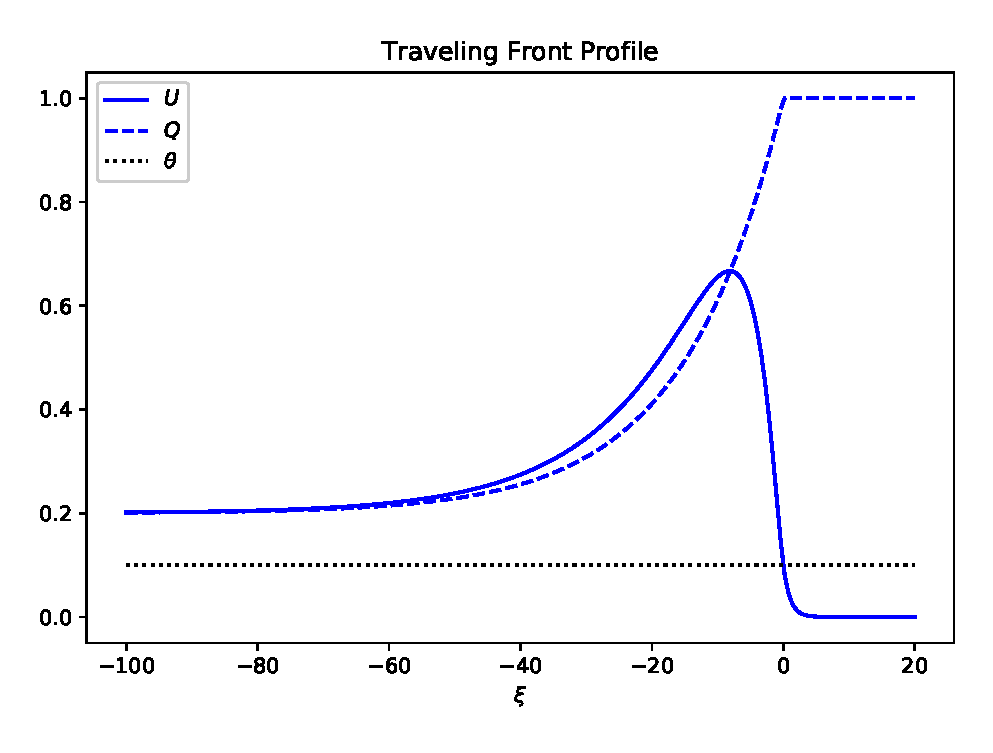
\includegraphics[width=.45\linewidth]{front_profile}
	\end{center}
	It also produces a consistancy condition which we can use to derive a formula for the front speed $c$. For $\theta < \gamma < 2\theta$ there are three solutions to the speed-consistency equation leading to three distict traveling front solutions: a regressive front with a negative speed, a slower unstable front and a faster stable front. The bifurcation diagram below below shows the front speed $c$ as determined by $\tau_q$ for a fixed $\theta = 0.1$, and highlights the pitchfork bifurcation occuring at $\gamma = 2\theta$.
	\begin{center}
		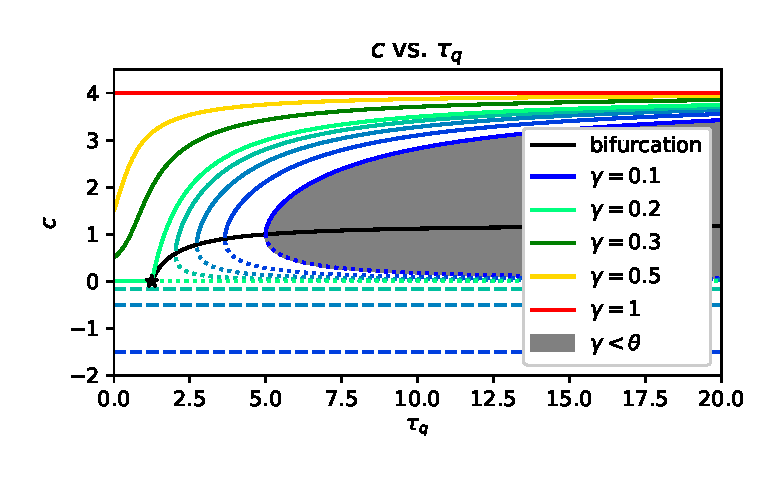
\includegraphics[width=.45\linewidth]{speed_by_tau_q}
	\end{center}
}

\headerbox{Traveling Pulse Solutions}{name=solutions2,column=1,below=solutions,above=bottom}
{
	The traveling pulse solutions have an active region given by $(-\Delta, 0)$ and similarly result in a decoupled system of linear equations.
	\begin{center}
		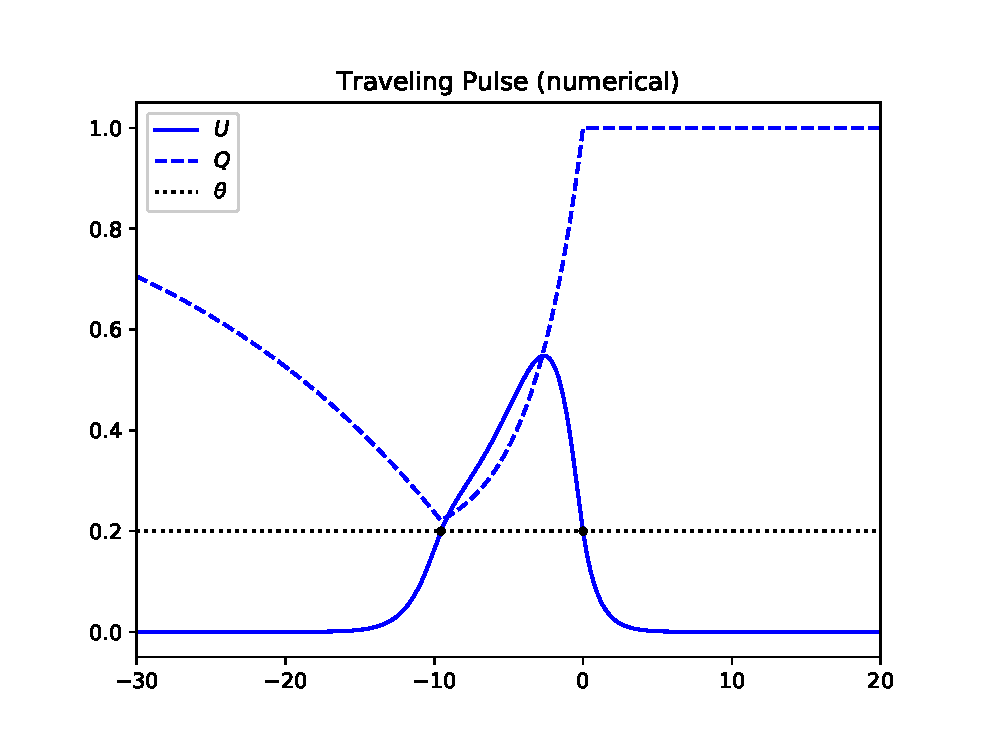
\includegraphics[width=.45\linewidth]{pulse_profile}
	\end{center}
	We also obtain two consistency equations for $c$ and $\Delta$, however, these equations cannot be found analytically so we resort to numerical root-finding techniques. The following diagram was generated using numerical continuation from a known solution that was found by trial and error.
	\begin{center}
		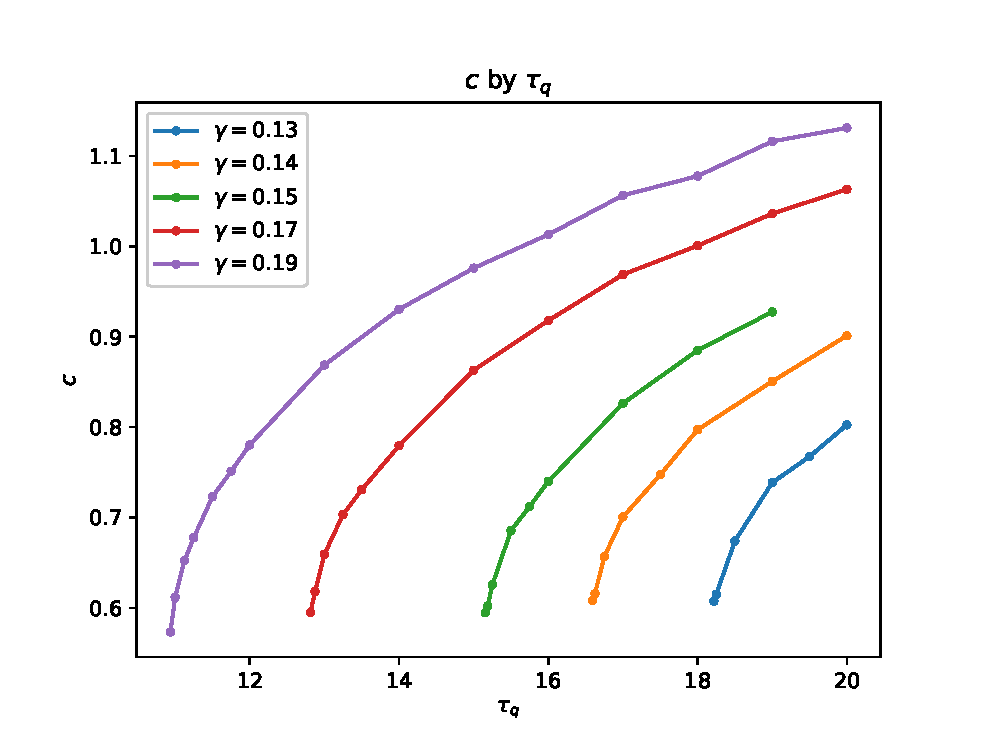
\includegraphics[width=.45\linewidth]{pulse_bifurcation}
	\end{center}
}

%%%%%%%%%%%%%%%%%%%%%%%%%%%%%%%%%%%%%%%%%%%%%%%%%%%%%%%%%%%%%%%%%%%%%%%%%%%%%%
\headerbox{Wave Response}{name=response,column=2,row=0,above=solutions2}
{
	These solutions have fixed speeds, however, our visual system is capable of tracking and predicting the location of objects with a variety of speeds. Can we augment the model in a biologically realisitc way to account for this variation in speed?
	\bigbreak
	
	We can model stimulii from other areas of the brain as forcing terms $I_u, I_q$ in our model:
	\begin{align*}
		\tau_u u_t &= -u + w * (q f[u]) + \varepsilon I_u(x, t)\\
		\tau_q q_t &= 1 - q - \underbrace{(\tfrac{1}{\gamma} - 1)}_{\beta} q f[u] + \varepsilon I_q(x, t)
	\end{align*}
	Below we see the effects of choosing $I_q = 0$ and $\varepsilon I_u = 0.1 \delta(t-20)$. That is, at time $t=20$, we instantainously stimulate the activity variable over the entire spatial domain. We see that the profile of the pulse deforms slightly after, but that deformation is transient, and the solution tends towards a translate of the original traveling pulse solution. 
	\begin{center}
		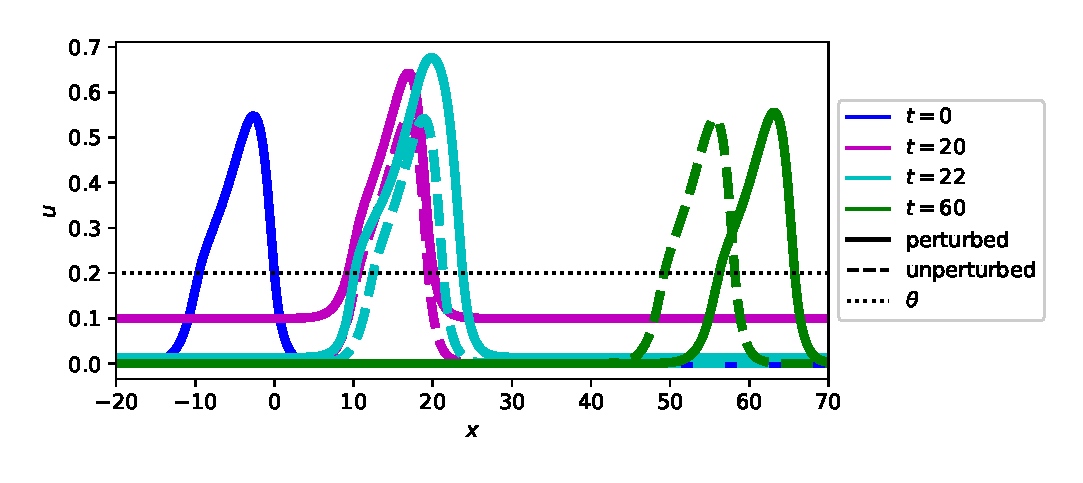
\includegraphics[width=.7\linewidth]{response_example}
	\end{center}
	This is called \textit{marginal stability}. The amount of translation is called the \textit{wave response}, denoted $\nu(t)$, and is a function of time, and the particular stimulus functions. An animation of this phenomeneon can be found in the online supplemental material (QR code).
	\vspace{.2cm}
}

%%%%%%%%%%%%%%%%%%%%%%%%%%%%%%%%%%%%%%%%%%%%%%%%%%%%%%%%%%%%%%%%%%%%%%%%%%%%%%
\headerbox{Asymptotics}{name=asymptotics,column=2,below=solutions,above=bottom}
{
	We can explore the effects of small perturbations by taking $\varepsilon$ to be small and linearlizing about the traveling wave solution:
	\begin{align*}
		u(\xi, t) &= U(\xi - \varepsilon \nu(t)) + \epsilon \phi(\xi, t) + \OO(\varepsilon^2) \\
		q(\xi, t) &= Q(\xi - \varepsilon \nu(t)) + \epsilon \psi(\xi, t) + \OO(\varepsilon^2)
	\end{align*}
	When substituted into the model, the $\OO(1)$ terms are consistent with $U, Q$ being a traveling wave solution, and the $\OO(\varepsilon)$ terms can collected and expressed in vector form as
	\begin{align*}
	    \begin{bmatrix}\tau_u & 0 \\ 0 & \tau_q\end{bmatrix} \begin{bmatrix}\phi \\ \psi \end{bmatrix}_t + \LL \left(\begin{bmatrix} \phi \\ \psi \end{bmatrix} \right)
	        = 
	        \begin{bmatrix} I_u + \tau_u U' \nu' \\ I_q + \tau_q Q' \nu ' \end{bmatrix}
	\end{align*}
	where
	\begin{align*}
	\LL \left(\begin{bmatrix} \phi \\ \psi \end{bmatrix} \right) = \begin{bmatrix}\phi \\ \psi \end{bmatrix} - c\begin{bmatrix}\tau_u & 0 \\ 0 & \tau_q\end{bmatrix} \begin{bmatrix}\phi \\ \psi \end{bmatrix}_\xi +
	\begin{bmatrix}
	   -w Q f'(U) * \cdot  & -w f(U) * \cdot \\
	   \beta Q f'(U) & \beta f(U)
	\end{bmatrix}
	\begin{bmatrix}\phi \\ \psi \end{bmatrix}
	\end{align*}
	is a linear integro-differential operator.
	\bigbreak
	
	A unique bounded solution exists if the right-hand-side is orthogonal to the null-space of the adjoint of the linear operator. For $(v_1, v_2) \in \mathcal{N}(\LL^*)$, 
	\[
		\nu(t) = - \frac{\int_\RR v_1 \int_0^t I_u(\xi, \tau) \ d\tau + v_2 \int_0^t I_q(\xi, \tau) \ d\tau \ d\xi}{\int_\RR \tau_u U' v_1 + \tau_q Q' v_2 \ d\xi}.
	\]
	This null-space can be found analytically with respect to the traveling wave solution and speed/width parameters.
	\vspace{.2cm}
}

%%%%%%%%%%%%%%%%%%%%%%%%%%%%%%%%%%%%%%%%%%%%%%%%%%%%%%%%%%%%%%%%%%%%%%%%%%%%%%
\headerbox{Results}{name=results,column=3,row=0}
{
	In the case of a traveling front, we find the null-space to be
	\begin{align*}
		v_1(\xi) &= H(\xi) e^{-\xi/c\tau_u} \\
		v_2(\xi) &= \frac{c\tau_u}{2(1+c\tau_u)(1+\beta+c\tau_q)} \big( H(-\xi)e^{\xi} + H(\xi) e^{-\xi/c\tau_q} \big)
	\end{align*}
	which is depicted below for a large (biologically realistic) value of $\tau_q$.
	\begin{center}
		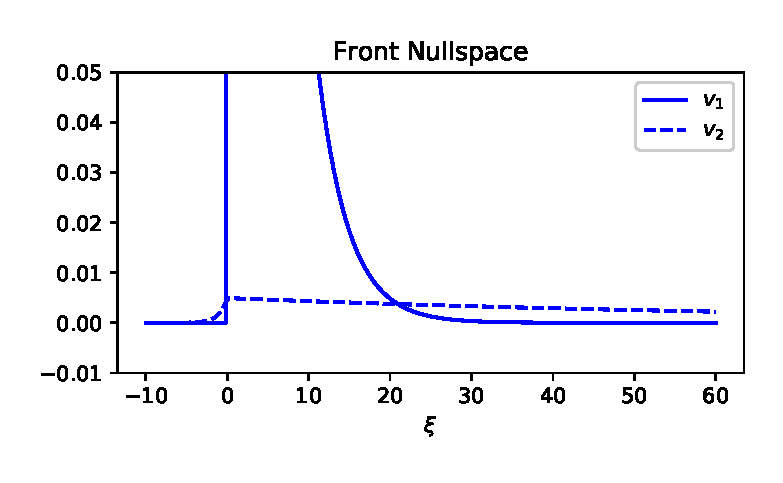
\includegraphics[width=.9\linewidth]{nullspace}
	\end{center}
	The profile of the nullspace is a useful heuristic. For example, we see that far in front of the wave, $\xi \approx 50$ for example, $v_1 \approx 0$ while $v_2 > 0$. This suggests that if we were to add some localized stimulus $I_u$ it would have no effect, while a stimulus $I_q$ would persist long enough to cause a wave response.
	\bigbreak
	
	Do demonstrate how the asymptotic prediction of the time limit $\lim\limits_{t \to \infty} \nu(t) = \nu_\infty$ compares to simulation, we consider the stimulus $\varepsilon I_u = \varepsilon \delta_t$ with $I_q = 0$.
	\begin{center}
		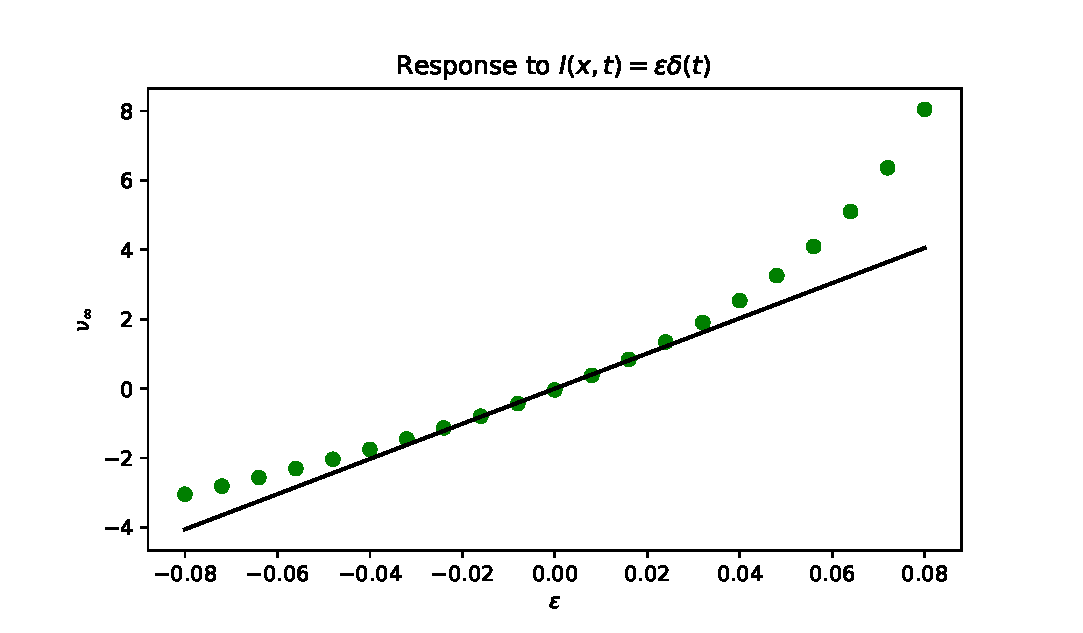
\includegraphics[width=.9\linewidth]{fig_spatially_homogeneous_limit}
	\end{center}
	We see that the predicted response function is tangent to the observed response from simulations, and accurately predicts the response for small stimulii, as one expects of an asymptotic approximation.
	\vspace{.2cm}
}

%%%%%%%%%%%%%%%%%%%%%%%%%%%%%%%%%%%%%%%%%%%%%%%%%%%%%%%%%%%%%%%%%%%%%%%%%%%%%%
\headerbox{References, Funding, and Links}{name=references,column=3,below=results,above=bottom}
{
	\begin{itemize}
		\item Z. Kilpatrick \& P. Bressloff. ``Effects of synaptic depression and adaptation on
		spatiotemporal dynamics of an excitatory neuronal network''. Physica D (2010)
		\item Z. Kilpatrick \& B. Ermentrout. ``Response of traveling waves to transient inputs in
		neural fields''. Phys. Rev. E( 2012)
	\end{itemize}
}

\end{poster}
\end{document}
